\subsection{Sensor > Ground-Based Lidar > Show depth buffer}
\label{subsection:showGBLDepthBuffer}

\index{profondeur, carte de}
\index{capteur}

\begin{figure}[!h]
\begin{center}
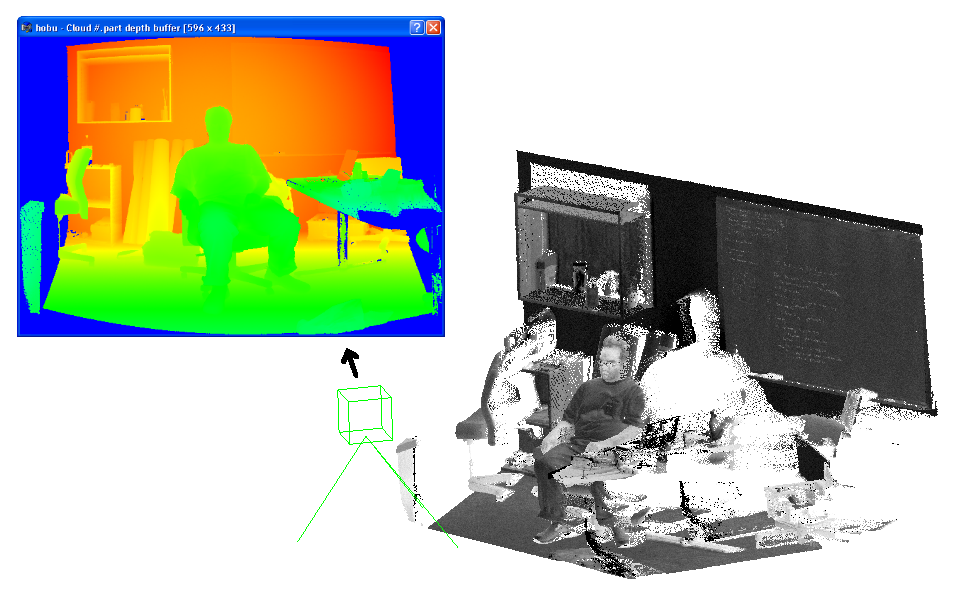
\includegraphics[width=0.7\textwidth]{Partie3_Fonctions/gblDepthBuffer.png}
\caption{\label{fig:gblDepthBuffer}Carte de profondeur associ�e � une entit� scanner (\textit{GBL sensor})}
\end{center}
\end{figure}


Affiche la carte de profondeur associ�e � un \emph{capteur} (GBL sensor - voir figure~\ref{fig:depthBuffer}). Elle correspond aux points 3D affich�s en fausses couleurs (en fonction de la distance par rapport au capteur) et projet�s dans le repaire polaire du scanner (li� � la rotation des mirroirs).
